


\documentclass[a4paper,10pt]{article}
\usepackage{listings,color,epsfig,amsmath,url}
\definecolor{codecolor}{rgb}{0.99,0.97,0.94} % color values Red, Green, Blue
\definecolor{commentcolor}{rgb}{0.1,0.5,0.1} % color values Red, Green, Blue
\definecolor{stringcolor}{rgb}{0.3,0.1,0.1} % color values Red, Green, Blue
\newcommand{\Code}[1]{\texttt{#1} }
\newcommand{\code}[1]{\Code{#1} }
\newcommand{\DB}   {\code{{MOOSDB}}}
\newcommand{\MA}   {\code{{MOOSApp}}}
\newcommand{\Ignore}[1]   {}



% Title Page
\title{Graphical Tools: \code{uMS} and \code{uPB}}
\author{Paul Newman}


\begin{document}
\maketitle

\begin{center}

\epsfig{file=images/moose6.eps,width = 0.2\linewidth}
\end{center}
\begin{abstract}
This document will give you a description of two graphical tools: MOOScope (\code{uMS}) and Playback (\code{uPB}).
\end{abstract}


\section{Visual Debugging - \code{uMS}}\label{sec:MOOSScope}
The \code{uMS} is another GUI application. It allows a user to
place a stethoscope on the MOOS network and watch what variables
are being written, which processes are writing them, and how often
this is happening. After starting up the scope and specifying the
host name and port number of the \DB the user is presented with a
list of all MOOS variables in the server and their current state.
Several times a second \code{uMS} calls into the DB and uses a
special/unusual (and intentionally undocumented) message that
requests that the server inform the client about {\em{all}}
variables currently stored along with their update statistics.
\code{uMS} is a central tool in the MOOS suite. It is cross-platform and should
be used to spy on and present visual feedback
on any MOOS community.

\begin{figure}
\center 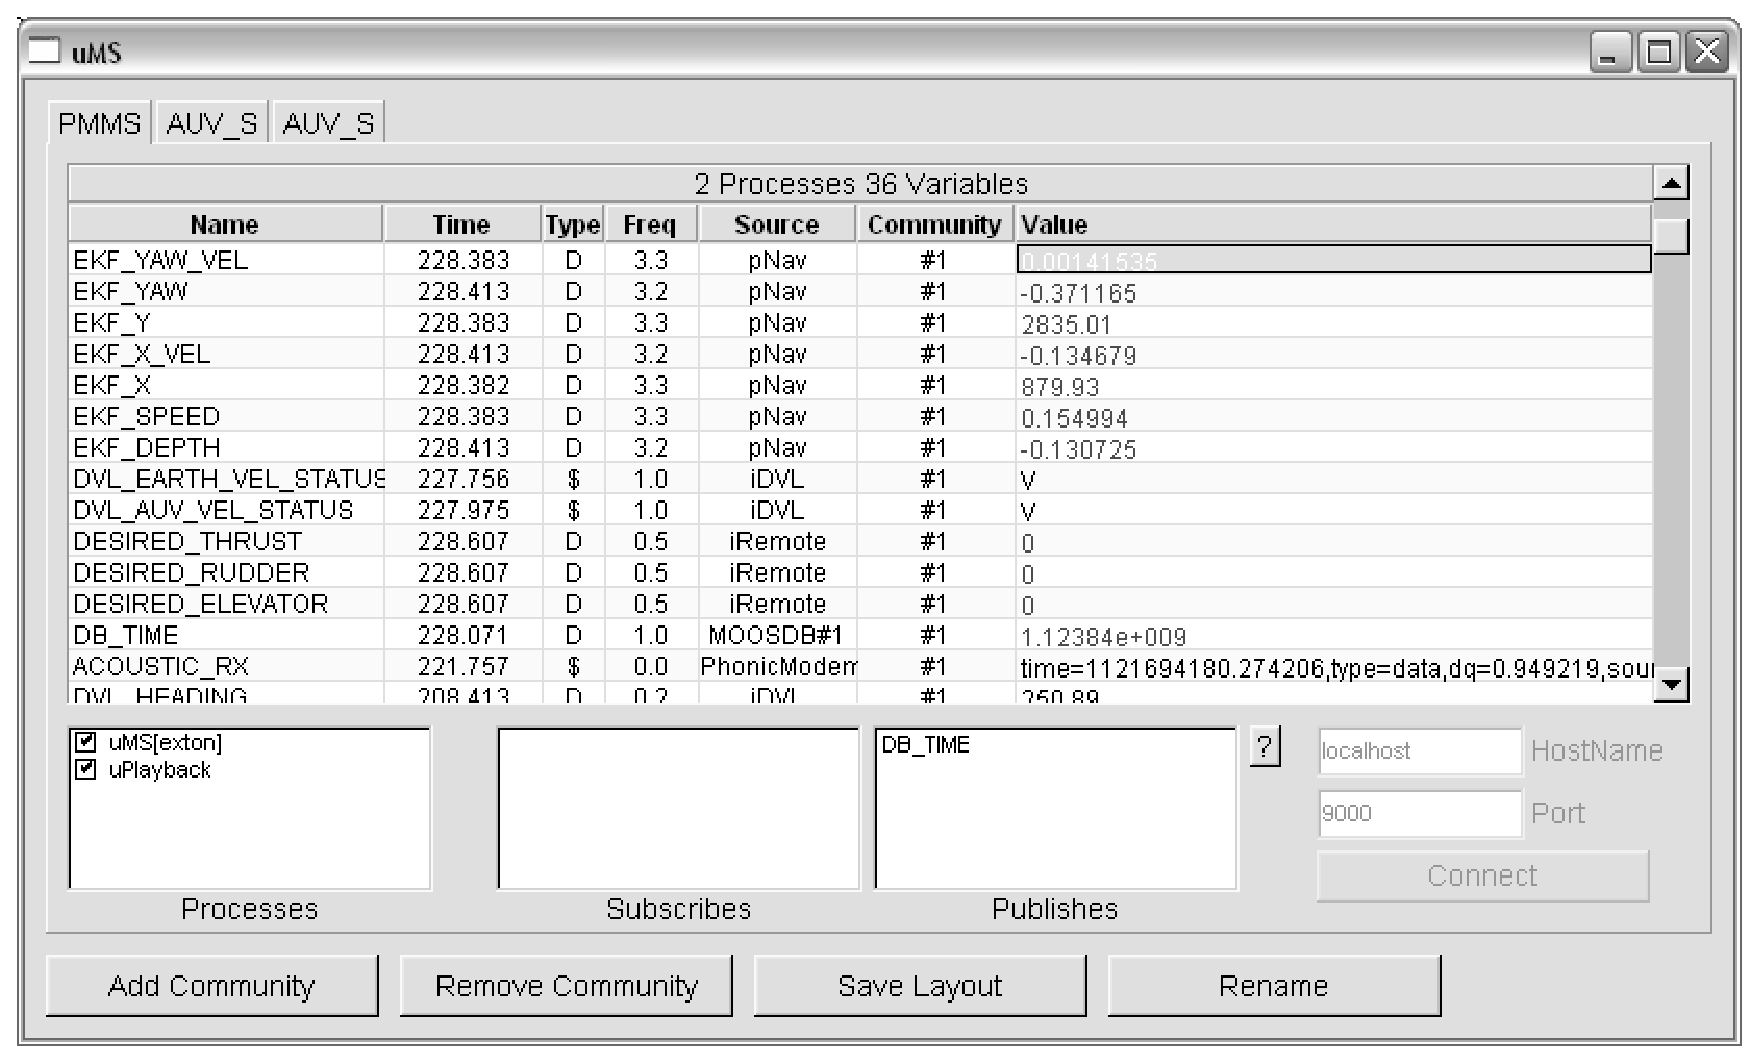
\epsfig{file=images/uMS.eps,width = 1.0\linewidth} \caption{A
screen shot of \code{uMS} -- a cross-platform, multi-community MOOS Comms
viewer.}
\end{figure}

\subsection{Functionality Summary}

Hopefully it will be pretty obvious how to use \code{uMS} as soon as you run it up. But here is a quick summary.

\begin{itemize}
    \item Support for multiple communities via tabbed GUI.
    \item Memory of last settings (persistence).
    \item String expansion (click on long data strings and balloon
    appears).
    \item Show/hide unassigned variables.
\item View subscriptions and publications on a per process basis by clicking on the process list.	
    \item Show/hide messages from specific processes
    (shift-leftclick on the process list).
    \item Poke the MOOS via ctrl-leftclick on a variable or empty
    cell (see Section\ref{Sec:Poke}).
\end{itemize}

\subsection{Poking the MOOS}\label{Sec:Poke}
\code{uMS} has one other valuable use: poking the MOOS. It allows
a user to double-click on a variable name and alter its value
(string or double) interactively. This is akin to changing memory
contents in a source code debugging session. The difference here
is that this action is a notification and all clients that are
registered for it receive a message in their mail box and act on
it accordingly. The utility of this functionality should not be
underestimated. For example, during the commissioning of a new
sensor (say a DVL) it may be unclear what the best configuration
parameters are. For example, by having the managing process
subscribe for notifications on a \code{PARAMETERS} variable the
\code{uMS} can be used to rapidly explore the
performance/parameter space by simply poking new configuration-
describing strings into the \code{PARAMETERS} variable.


\section{Replay with \code{uPB}}
There is a FLTK-based, cross-platform GUI application that can
load in {\it{alog}} files and replay them into a MOOS community as
though the originators of the data were really running and issuing
notifications. A typical use of this application is to ``fake''
the presence of sensor processes when reprocessing sensor data and
tuning navigation filters. Alternatively it can be used in pure
replay mode, perhaps to render a movie of the recorded mission. The
GUI allows the selection of which processes are ``faked''. Only
data recorded from those applications will be replayed from the
log files.  There is a single class that encapsulates all the
replay functionality -- \code{CMOOSPlayback}. The GUI simply hooks
into the methods exported by this class. The GUI is almost self
documenting -- start it up and hold the mouse over various buttons
and hint balloons will appear, telling you what each button does.

\begin{figure}
\center 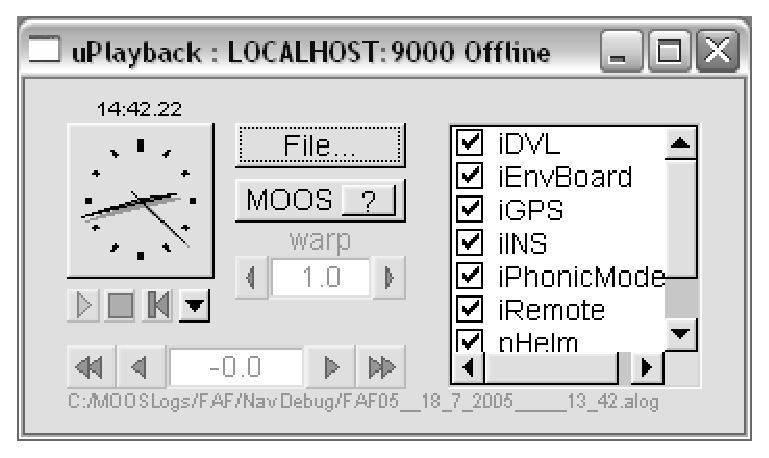
\epsfig{file=images/uPB.eps,width = 0.5\linewidth} \caption{A
screen shot of \code{uPB} -- a cross-platform ``alog'' playback
tool}
\end{figure}

\subsection{Controlling Playback Rate Progammatically}

A client process can control the replay of MOOS messages by
writing to the \code{PLAYBACK\_CHOKE} variable and writing a valid
time in the numeric message field. The Playback executable will
not play more than a few seconds past this value before waiting
for a new value to be written. In this way it is possible to
debug (halt inspect and compile-in-place etc) at source level a
client application using replayed data, without having the playback
rush on ahead during periods of thought or code-stepping.



\end{document} 